%% LyX 2.3.4.2 created this file.  For more info, see http://www.lyx.org/.
%% Do not edit unless you really know what you are doing.
\documentclass[english]{article}
\usepackage[T1]{fontenc}
\usepackage[latin9]{inputenc}
\usepackage{geometry}
\geometry{verbose,tmargin=3cm,bmargin=3cm,lmargin=3cm,rmargin=3cm}
\usepackage{babel}
\usepackage{verbatim}
\usepackage{float}
\usepackage{amsmath}
\usepackage{amssymb}
\usepackage{graphicx}
\usepackage[unicode=true,
 bookmarks=false,
 breaklinks=false,pdfborder={0 0 1},backref=section,colorlinks=false]
 {hyperref}

\makeatletter
%%%%%%%%%%%%%%%%%%%%%%%%%%%%%% User specified LaTeX commands.
\usepackage{babel}

\makeatother

\begin{document}
\title{\textbf{Introduction to Gaussian Process}}
\author{Matheus Schossler}

\maketitle
\begin{comment}
Let $\left\{ f(x):x\in\mathcal{X}\right\} $ be a collection of of
random variables indexed by elements from some set $\mathcal{X}$. 
\end{comment}
{} A \textbf{Gaussian process} are used to define probability distribution
over functions. With this concept, we can build the Gaussian process
regression algorithm (GPR), which is a data-based prediction method
with good performance in dealing with high dimension small samples,
nonlinear problems. Let us start with a simpler algorithm to build
our intuition around Gaussian processes: the Bayesian linear regression.

\subsection*{Bayesian Linear Regression}

Let $S=\left\{ \left(x^{(i)},y^{(i)}\right)\right\} _{i=1}^{m}$be
a training set of i.i.d. examples from a unknown distribution. The
linear regression states that

\begin{equation}
y^{(i)}=\theta^{T}x^{(i)}+\varepsilon\label{1}
\end{equation}
where $\varepsilon$ are i.i.d. noise with $\mathcal{N}\left(0,\sigma^{2}\right)$
distribution. This implies

\begin{equation}
p\left(y^{(i)}|x^{(i)},\theta\right)=\frac{1}{\sqrt{2\pi}\sigma}\exp\left(-\frac{y^{(i)}-\theta^{T}x^{(i)}}{2\sigma^{2}}\right).\label{2}
\end{equation}
In Bayesian linear regression, we assume a \textbf{prior distribution}
over parameters is also given,

\begin{equation}
\theta\sim\mathcal{N}\left(0,\tau^{2}I\right),
\end{equation}
which from Bayes's rule, the $\theta$ distribution conditioned to
$S$ is

\begin{equation}
p(\theta|S)=\frac{p(\theta)p(S|\theta)}{\int_{\theta'}p(\theta')p(S|\theta')d\theta'}.
\end{equation}
In this model $p(S|\theta)=\prod_{i}p\left(y^{(i)}|x^{(i)},\theta\right)$,
where $p\left(y^{(i)}|x^{(i)},\theta\right)$ is the normal distribution
defined in \ref{2}. The output of this model on a new test point
$x_{*}$is given by the \textbf{posterior predictive distribution}

\begin{equation}
p(y_{*}|x_{*},S)=\int_{\theta}p(y_{*}|x_{*},\theta)p(\theta|S)d\theta.
\end{equation}
For the linear regression model above, we can express both $p(\theta|S)$
and $p(y_{*}|x_{*},S)$ in terms of a closed formula of $X_{*},S,\sigma,\tau$.
It can be shown that BLR is a GPR with the kernel given by the Dot-Product.

\subsection*{Gaussian Process}

A Gaussian Process is a collection of random variables, any finite
number of which have (consistent) joint Gaussian distributions. A
Gaussian process is fully specified by its mean function $m(x)$ and
covariance function $k(x,x')$: 
\begin{equation}
f\sim\mathcal{GP}(m,k),
\end{equation}
which reads ``the function $f$ is distributed as a GP with mean
function $m$ and covariance function $k$''. We use a set of indexes
$\{x_{i}\in\mathcal{X}\}_{i=1}^{m}$ to denote the equation above
in terms of their vector notation \textbf{$\boldsymbol{f}$}:

\begin{equation}
\left[\begin{array}{c}
f(x_{1})\\
\vdots\\
f(x_{m})
\end{array}\right]\sim\mathcal{N}\left(\left[\begin{array}{c}
m(x_{1})\\
\vdots\\
m(x_{m})
\end{array}\right],\left[\begin{array}{ccc}
k(x_{1},x_{1}) & \cdots & k(x_{1},x_{m})\\
\vdots & \ddots & \vdots\\
k(x_{m},x_{1}) & \cdots & k(x_{m},x_{m})
\end{array}\right]\right),
\end{equation}
where $\mathcal{N}\left(\mu,\Sigma\right)$ denotes a multivariate
Gaussian distribution with mean $\mu\in\mathbb{R}^{n}$ and covariance
matrix $\Sigma$ as defined above.

\subsubsection*{Example}

The Bayesian linear model suffers from limited expressiveness. A very
simple idea to overcome this problem is to project the inputs into
some high dimensional space using a set of basis feature space functions,
e.g. $\left\{ 1,x,x^{2},\ldots,x^{d-1}\right\} $, and then apply
the linear model in this space instead of directly on the inputs themselves.
This type of map also defines a simple example of a Gaussian process:

\begin{equation}
f(\boldsymbol{x})=\phi\left(\boldsymbol{x}\right)^{T}\boldsymbol{\theta}
\end{equation}
where $\boldsymbol{x}$ is a $p$ variable input, $\phi\left(\boldsymbol{x}\right)$
is a $p\times d$ dimension vector, and the prior $\boldsymbol{\theta}\sim\mathcal{N}\left(\boldsymbol{0},\Sigma_{p}\right)$,
where $\Sigma_{p}$ is a a $p\times p$ covariance matrix, which implies
\begin{align}
\mathbb{E}[f(\boldsymbol{x})] & =\phi\left(\boldsymbol{x}\right)^{T}\mathbb{E}[\boldsymbol{\theta}]=0\nonumber \\
\mathbb{E}[f(\boldsymbol{x})f(\boldsymbol{x}')] & =\phi\left(\boldsymbol{x}\right)^{T}\mathbb{E}[\boldsymbol{\theta}\boldsymbol{\theta}^{T}]\phi\left(\boldsymbol{x}'\right)=\phi\left(\boldsymbol{x}\right)^{T}\Sigma_{p}\phi\left(\boldsymbol{x}'\right).
\end{align}
$f(\boldsymbol{x})$ and $f(\boldsymbol{x}')$ are jointly Gaussian
with zero mean and covariance $k(\boldsymbol{x},\boldsymbol{x}')=\phi\left(\boldsymbol{x}\right)^{T}\Sigma_{p}\phi\left(\boldsymbol{x}'\right)$.
Therefore any combination of $f(\boldsymbol{x}^{(i)})$, with $\boldsymbol{x}^{(i)}$
in the input set $X$ is a Gaussian process. Using the kernel trick
it is possible to show that, fundamentally all we need to know about
the feature map $\phi\left(\boldsymbol{x}\right)$ is encapsulated
in the corresponding kernel function $k(\boldsymbol{x},\boldsymbol{x}')\ (=\Sigma_{p})$.
We only need to specify weighted inner products of the feature space
and never need to specify the feature space.

\subsection*{Gaussian Process Regression}

Gaussian process regression (GPR) is a typical data-based prediction
method, which has a better performance in dealing with \textbf{high
dimension small sample}, \textbf{nonlinear} \textbf{problems}. GPR
uses the kernel to define the covariance of a prior distribution over
the target functions and uses the observed training data to define
a likelihood function. Based on Bayes theorem, a (Gaussian) posterior
distribution over target functions is defined, whose mean is used
for prediction. Let $S=\left\{ \left(x^{(i)},y^{(i)}\right)\right\} _{i=1}^{m}$
be a training set of i.i.d. examples from an unknown distribution.
A noisy regression algorithm problem is concerned with estimating
a function $f$ such that 
\begin{equation}
y^{(i)}=f\left(x^{(i)}\right)+\varepsilon,\ i=1,\ldots,m
\end{equation}
where $\varepsilon$ are i.i.d. noise with $\mathcal{N}\left(0,\sigma^{2}\right)$
distribution.

We assume a \textbf{prior distribution} over functions $f(\cdot)$
following a zero-mean Gaussian process

\begin{equation}
f\sim\mathcal{GP}(0,k),
\end{equation}
for some valid covariance function (or kernel) $k(\cdot,\cdot)$.
It can be shown that the squared-exponential covariance function 
\begin{equation}
k(\boldsymbol{x},\boldsymbol{x}')=\sigma_{f}\exp\left(-\frac{1}{2l^{2}}||\boldsymbol{x}-\boldsymbol{x}'||^{2}\right),
\end{equation}
where $\sigma_{f}$ and $l$ are the hyperparameters, corresponds
to a Bayesian linear regression model with an infinite dimensional
basis (we can make the train data set as large as we want and the
space the kernel operates in keeps growing without bound).

Now, let $T=\left\{ \left(x_{*}^{(i)},y_{*}^{(i)}\right)\right\} _{i=1}^{m}$be
a test set of i.i.d. examples from the same unknown distribution as
$S$. We want to calculate the posterior predictive distribution over
the testing outputs $y_{*}^{(i)}$. We write the joint distribution
of both sets $\left\{ f(x):x\in X\right\} $ and $\left\{ f_{*}(x):x\in X_{*}\right\} $
\begin{equation}
\left[\begin{array}{c}
\boldsymbol{f}\\
\boldsymbol{f_{*}}
\end{array}\right]|X,X_{*}\sim\mathcal{N}\left(0,\left[\begin{array}{cc}
K(X,X) & K(X,X_{*})\\
K(X_{*},X) & K(X_{*},X_{*})
\end{array}\right]\right)\Rightarrow\boldsymbol{f_{*}}|\boldsymbol{f}\sim\text{Normal distribution}.
\end{equation}
Using the formula for conditioning a joint Gaussian distribution we
can find an expression for $\boldsymbol{f_{*}}|\boldsymbol{f}$. The
joint Gaussian i.i.d. noise vector becomes 
\begin{equation}
\left[\begin{array}{c}
\boldsymbol{\varepsilon}\\
\boldsymbol{\varepsilon_{*}}
\end{array}\right]|X,X_{*}\sim\mathcal{N}\left(0,\left[\begin{array}{cc}
\sigma^{2}I & 0\\
0 & \sigma^{2}I
\end{array}\right]\right).
\end{equation}
Finally the \textbf{posterior predictive distribution} is found, 
\begin{align}
\left[\begin{array}{c}
\boldsymbol{y}\\
\boldsymbol{y_{*}}
\end{array}\right]|X,X_{*} & =\left[\begin{array}{c}
\boldsymbol{f}\\
\boldsymbol{f_{*}}
\end{array}\right]+\left[\begin{array}{c}
\boldsymbol{\varepsilon}\\
\boldsymbol{\varepsilon_{*}}
\end{array}\right]\sim\mathcal{N}\left(0,\left[\begin{array}{cc}
K(X,X)+\sigma^{2}I & K(X,X_{*})\\
K(X_{*},X) & K(X_{*},X_{*})+\sigma^{2}I
\end{array}\right]\right).\\
 & \Rightarrow
\end{align}
\begin{equation}
\boxed{\boldsymbol{y_{*}}|\boldsymbol{y},X,X_{*}\sim\mathcal{N}\left(\mu_{*},\Sigma_{*}\right)}
\end{equation}
Where $\mu_{*},\Sigma_{*}$ are expressed in terms of $X_{*},S,k(\cdot,\cdot),\sigma$
\begin{align}
\mu_{*} & =K(X_{*},X)\varLambda^{-1}\boldsymbol{y}\\
\Sigma_{*} & =K(X_{*},X_{*})-K(X_{*},X)\varLambda^{-1}K(X_{*},X),
\end{align}
where $\varLambda=K(X,X)+\sigma^{2}I$.

\subsection*{Bayesian Linear Regression as a Gaussian Process Regressor}

A Gaussian process $f(x)$ is completely specified by its mean function
$m(x)$ and covariance function $k(x,x\prime)$. Here $x\in X$ denotes
a point on the index set $X$. These functions are defined by

\begin{equation}
m(x)=\mathbb{E}[f(x)]
\end{equation}
and 
\begin{equation}
k(x,x\prime)=\mathbb{E}[(f(x)-m(x))(f(x\prime)-m(x\prime))].
\end{equation}
Ref \href{https://juanitorduz.github.io/reg_bayesian_regression/}{link}shows
that $f(x)$ as defined by (\ref{1}) defines a Gaussian Process because
$\theta\sim\mathcal{N}\left(0,\tau^{2}I\right)$. In addition, \href{https://stats.stackexchange.com/questions/507527/bayesian-linear-regression-as-a-gaussian-process}{link},
shows that $m(x)=0$ and $k(x,x\prime)=\tau^{2}x^{T}x+\sigma^{2}.$%
\begin{comment}

\subsubsection*{Example }

As an example of linear function we use 
\begin{equation}
f(x)=0.4x+10,
\end{equation}
on the range $x\in[0,100]$ for train data and $x\in[0,150]$ for
test data. We generate both train and test data utilizing this function
with white noise $\epsilon=\mathcal{N}\left(0,\sigma^{2}\right)$,
where $\sigma=1$. 
\end{comment}


\subsection*{Training a Gaussian Process Regressor}

Gaussian Process Regressor is useful if we have enough prior information
about a dataset at hand to specify prior mean and covariance functions
confidently. However, the availability of such detailed prior information
is not the typical case in machine learning applications. We use hierarchical
specification to specify vague prior information in the form of $m$
and $k$ in a simple way and optimize the introduced hyperparameters
based on the data.

We start writing a general model: 
\begin{equation}
f\sim\mathcal{GP}(m,k),
\end{equation}
where 
\begin{align}
m(\boldsymbol{x}) & =a\boldsymbol{x}^{2}+b\boldsymbol{x}+c\\
k(\boldsymbol{x},\boldsymbol{x}') & =\sigma_{f}^{2}\text{exp}\left(-\frac{^{2}}{2l^{2}}\left(\boldsymbol{x}-\boldsymbol{x}'\right)^{T}M\left(\boldsymbol{x}-\boldsymbol{x}'\right)\right)+\sigma_{n}^{2}\delta_{ii'}
\end{align}
we define the hyperparameters set as : 
\begin{equation}
H=\{a,b,c,\{M\},\sigma_{f},\sigma_{n}\},
\end{equation}
where $M$ can be defined in terms of the characteristic length-scales
of correlations, $l_{i}$, or the factor analysis distance matrix,
$\varLambda$. For high-dimensional datasets, this matrix could identify
a few directions in the input space with especially high "relevance"
(in the sense of PCA - high variance). Although we are using squared
exponential, any positive definite function can be used as covariance
function.

Given the marginal likelihood 
\begin{align}
L & =\log p(\boldsymbol{y}|\boldsymbol{x},f)=-\frac{1}{2}\left(\log|\Sigma|+\left(\boldsymbol{y}-m\right)^{T}\Sigma^{-1}\left(\boldsymbol{y}-m\right)\right)
\end{align}
we can maximize $L$ using its partial derivatives with respect to
$H$: 
\begin{equation}
\frac{\partial L}{\partial H_{m}},\frac{\partial L}{\partial H_{k}},
\end{equation}
where $H_{m}$ and $H_{k}$ are used to indicate hyperparameters of
the mean and covariance functions, respectively, and optimization
algorithms such as the gradient descent, momentum gradient descent,
or the Adam algorithm.

The trade-off between penalty and data fit in the GP model is automatic
(based on the $L$ exact expression). %
\begin{comment}
There is no weighting parameter which needs to be set by some external
method such as cross validation. 
\end{comment}


\subsection*{Disadvantages of Gaussian Process Regression}
\begin{itemize}
\item It is expensive to build a model when there is a lot of training data.
An implementation of the algorithm explained here requires the inversion
of the covariance matrix $\Sigma=K(X,X)$ using (Cholesky factorization),
with a memory complexity of $O(n^{2})$ and a computational complexity
of $O(n^{3})$. There has been work on GP models that only include
a \textbf{subset of the data} (Gramacy and Apley 2015) which can be
implemented efficiently (Gramacy et al. 2014). 
\item Another issue of the model is stationary covariance function is assumed,
but for many problems, the character of the covariance function needs
to change in different regimes. Gramacy and Lee (2008) developed a
\textbf{hybrid tree-Gaussian process} \textbf{model} that allows the
covariance function to change over the range of input data. 
\end{itemize}

\subsubsection*{Alternatives}
\begin{itemize}
\item Alternatives of GPR are the Bayesian Multiple Adaptive Regression
Splines (\textbf{MARS}) which can automatically handle some of the
issues with nonstationary covariances, and the underlying computation
in fitting a Bayesian MARS model is a least-squares solve, which can
be done efficiently. 
\item The \textbf{twin Gaussian process} is a structured prediction method
which uses Gaussian process priors on both covariates and responses,
both multivariate. This method predicts outputs by minimizing the
Kullback-Leibler divergence between two GP modeled as normal distributions
over finite index sets of training and testing examples. It's based
on the fact that similar inputs should produce similar percepts. (Mohammad
Mojaddady, Moin Nabi, and Shahram Khadivi - Stock Market Prediction
using Twin Gaussian Process Regression). 
\begin{figure}[H]
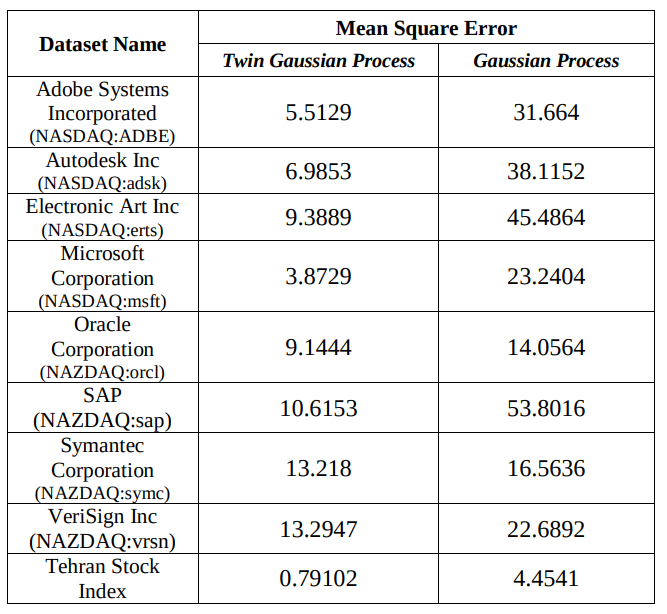
\includegraphics[scale=0.25]{figs/TGP_vs_GP_stocks}

\caption{Mean Square Error of Stock Market prediction}
\end{figure}
\item Use it together with other models (auto-encoder, recurrent neural
network (RNN) and long short-term memory (LSTM)) to construct the
interval prediction of the input signal and analyze the uncertainties
(e.g. stock market). \href{https://doi.org/10.1016/j.asoc.2021.107898}{Ref}:
Stock index prediction and uncertainty analysis using multi-scale
nonlinear ensemble paradigm of optimal feature extraction, two-stage
deep learning and Gaussian process regression, Wang et al. 2021. 
\end{itemize}
\begin{comment}
\[
f(x)=\sin(4\pi x)+\sin(7\pi x)
\]
\linebreak{}
\[
k(x,x')=\sigma_{f}\exp\left(-\frac{2\sin^{2}\left(\pi\Vert x-x'\Vert/p\right)}{l^{2}}\right),
\]
\end{comment}

\end{document}
